Модель Transformer является архитектурой глубокого обучения, предназначенной для обработки последовательных данных,
таких как тексты или временные ряды. 
Она была предложена в работе \cite{vaswani2017attention} и стала одной из наиболее инновационных архитектур
в области обработки естественного языка.

Основной компонент модели Transformer это механизм внимания. Он позволяет сфокусировать модель
на наиболее важных компонентах входных данных при выполнении таких задач, как машинный перевод или обработка текста.

\begin{figure}[h]
    \centering
    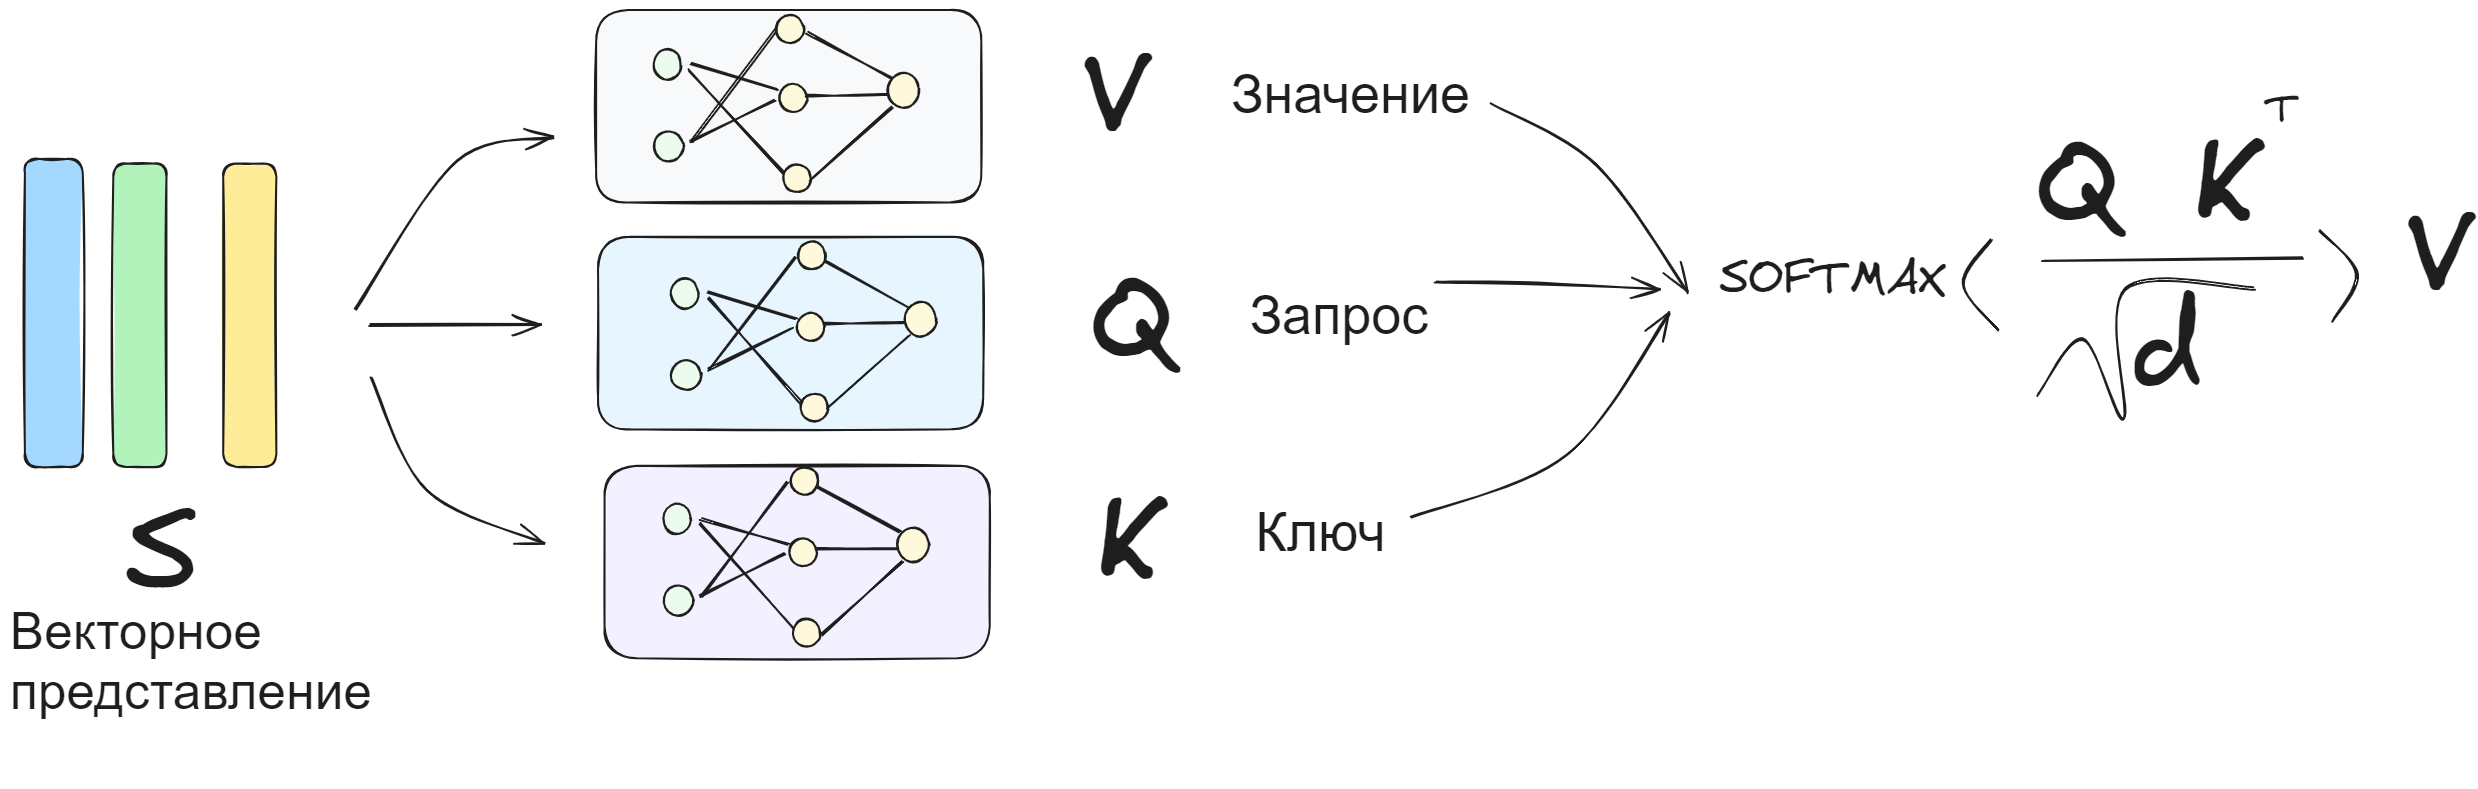
\includegraphics[width=0.7\textwidth]{assets/ml/nn/transformer.excalidraw.png}
    \caption{Механизм внимания в архитектуре Transformer \cite{vaswani2017attention}. }
    \label{attention}
\end{figure}

Расчет механизма внимания в архитектуре Transformer состоит из трех основных этапов:\begin{enumerate}
    \item  Расчет векторов запроса $q$, ключа $k$ и значения $v$.
    Они используются для вычисления весов входных данных и определения их важности для каждого элемента:
    \begin{equation}
        \begin{aligned}
            &q =W_q xб \\ 
            &k = W_k x, \\
            &v = W_v x,
        \end{aligned}
    \end{equation}
    где \(W_q\), \(W_k\), \(W_v\) --- матрицы весов, обучаемые моделью.
    \item Расчет логитов \(e_{ij}\):
    \begin{equation}
        e_{ij} = \frac{q \cdot k_j}{\sqrt{d_k}},
    \end{equation}
    где \(d_k\) --- длина запроса,
    \item Преобразование логитов в веса внимания \( \alpha_{ij} \) с помощью функции $\operatorname{softmax}$:
    \begin{equation}
        \alpha_{ij} = \frac{\exp(e_{ij})}{\sum_{j'} \exp(e_{ij'})}.
    \end{equation}
\end{enumerate}